\documentclass[./main.tex]{subfiles}

\begin{document}

\chapter{MAC interface}

\section{Principle concepts}

\begin{table}[ht]
    \centering
    \begin{tabularx}{\linewidth}{|c|L|L|} 
        \hline
        \textbf{Acronyms} & \multicolumn{1}{>{\centering}c|}{\textbf{Meaning}} &  \multicolumn{1}{>{\centering}c|}{\textbf{Explanation}}\\ 
        \hline
        PRF & Pulse Repetition Frequency & Indicates the number of pulses emitted by the transducer over a designated period of time. \\ 
        \hline
        SHR & Synchronization Header & Preamble + SFD \\
        \hline
        PPDU & PHY protocol data unit & Packet tranceived in physical layer\\
        \hline
    \end{tabularx}
    \caption{Principle concepts}
    \label{tab:uwb_ccp_blink_frame_t}
\end{table}

\section{Transmission duration}

\subsection{UWB physical attribute}
IEEE Std 802.15.4-2011\cite{IEEE_Std_802.15.4-2011} has defined the following physical attributes in table 101 (page 201):
\begin{itemize}
    \item $T_{psym}$: Preamble symbols duration, it is the duration of each symbols in preamble.
    \item $T_{bsym}$: Base rate symbols duration, it is the duration of each symbol in the physical header.
    \item $T_{dsym}$: Data rate symbols duration
    \item $N_{sfd}$: Number of symbols in start of frame delimiter
    \item $N_{sync}$: Number of symbols in preamble sequence
    \item $N_{phr}$: Number of symbols in phy header
\end{itemize}

Figure \ref{fig:UWB PPDU} shows the format of the UWB PPDU.
\begin{figure}[ht]
    \centering
    \begin{tabular}{ |M{0.2}|M{0.15}|M{0.5}|} 
        \hline
        \textbf{SHR Preamble} & \textbf{PHY Header (PHR)} & \textbf{Data field}\\
        \hline
    \end{tabular}
    \caption{UWB PPDU}
    \label{fig:UWB PPDU}
\end{figure}

\subsection{SHR and PHY header duration}

As illustrated in figure \ref{fig:SHR preamble structure}, the SHR duration $T_{pre}$ consists of two components:
\begin{itemize}
    \item SYNC duration $T_{sync}$ of preamble
    \item SFD duration $T_{sfd}$ of SFD
\end{itemize}
Thus, SHR duration can be calculated using the following formula:
% duration = ceilf(attrib->Tpsym * (attrib->nsync + attrib->nsfd));
\begin{equation}
    T_{pre} = T_{psym} * (N_{sync} + N_{sfd})
\end{equation}

\begin{figure}[ht]
    \begin{center}
        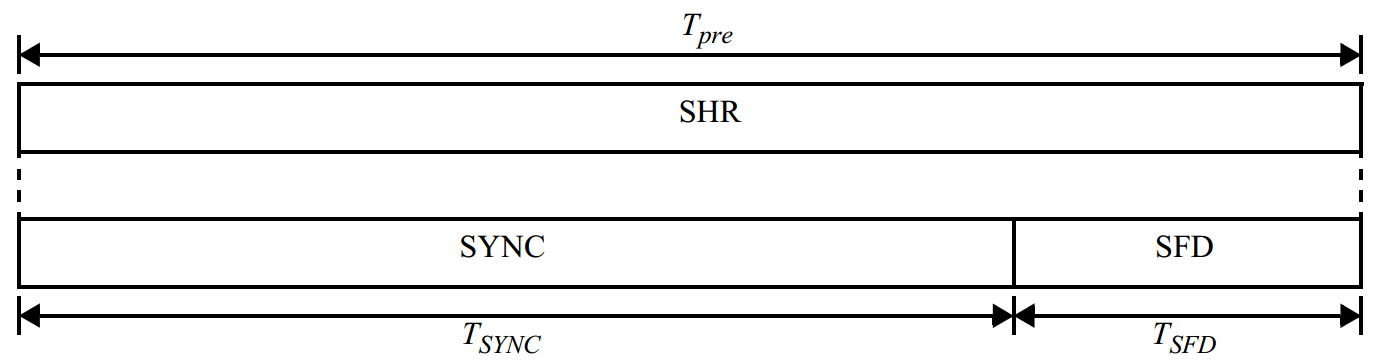
\includegraphics[scale=0.3]{SHR_preamble_structure}
    \end{center}
    \caption{SHR preamble structure}
    \label{fig:SHR preamble structure}
\end{figure}

Similarly, the PHY header duration is calculated using $T_{bsym}$ and $N_{phr}$:
\begin{equation}
    T_{phr} = T_{bsym} * N_{phr}
\end{equation}

\subsection{Data duration}
Because of the UWB PHY forward error correction, we need to add 48 parity bits for every 330 bits in the data payload (including CRC).
For example, if the number of data bit is less than 33, we need 48 parity bits, from 330 to 660, we need 48+48 parity bits, from 660 to 990, we need 3*48 parity bits, etc. So, with $nlen$ bytes  of data field (not include 2-byte CRC), the number of parity bit is:
% parity_data_bits += ((8*(nlen+2))/330) * 48;
\begin{equation}
    N_{parity\_data\_bit} = 48 + (int)((8*(nlen+2))/330) * 48;
\end{equation}
Actually, the total number of bits of data field transmitted is:
% total_payload_bits = 8*(nlen+2) + parity_data_bits;
\begin{equation}
    N_{total\_payload\_bit} = 8*(nlen+2) + N_{parity\_data\_bit};
\end{equation}
Since, each symbol represents one bit, the duration for data field is calculated as follow:
% duration = (int)ceilf(attrib->Tbsym * attrib->nphr + attrib->Tdsym * total_payload_bits);
\begin{equation}
    T_{dat} = T_{dsym} * N_{total\_payload\_bit}
\end{equation}

\underline{\textbf{Conclusion:}}
The total transmission duration for each packet transferred over the air is:
\begin{equation}
    T_{pak} = T_{pre} + T_{phr} + T_{dat}
\end{equation}

\section{Timestamp}

DW1000 includes a timing system with a 40 bits time counter register.

In TX and RX mode, system time and time stamps are designed to be based on the time units which are nominally at 64 GHz, or more precisely 499.2 MHz x 128 which is 63.8976 GHz. The counter wrap period of the clock is then: $2^{40} \div (128 \times 499.2 \times 10^6) = 17.2074$
seconds.

In idle mode with the digital PLL enabled, the System Time Counter is incremented at a rate of 125 MHz in units of 512. The nine low-order bits of this register are thus always zero. 

On power-up, before the digital PLL is enabled, the System Time Counter increments are still in units of 512 however the increment rate is half the external crystal frequency, (e.g. at 19.2 MHz for the 38.4 MHz crystal). The counter wrap period is then: $2^{31} \div 19.2 \times 10^6 = 111.8481$
seconds.

In sleep modes the system time counter is disabled and this register is not updated.

\subsection{Transmission timestamp}
During frame transmission, the start of the PHR (PHY header) is the event nominated by the IEEE 802.15.4 UWB PHY standard for message time-stamping. The time the first symbol of the PHR launches from the antenna (defined as the RMARKER) is the event nominated as the transmit time-stamp.

The DW1000 digital transmit circuitry takes note of the system clock counter as the RAW transmit timestamp at the point when it begins sending the PHR. It then adds to this the transmit antenna delay to get the antenna adjusted transmit timestamp that it writes to the TX\_STAMP field.

In performing a delayed transmission, the DW1000 calculates an internal start time for when to begin sending the preamble to make the RMARKER raw timestamp agree with the programmed transmit time. The DW1000 remains in idle state until the system time (Register file: 0x06 – System Time Counter) reaches the correct point to turn on the transmitter and begin preamble.

\end{document}
